\documentclass[10pt]{book} 

\usepackage{amsmath}
\usepackage{palatino}
\usepackage{parskip}
\usepackage{minted}
\usepackage[margin=1in,letterpaper]{geometry}
\usepackage{fancyvrb}
\usepackage{color}
\definecolor{maroon}{RGB}{66,00,00}

\usepackage{hyperref}
% http://en.wikibooks.org/wiki/LaTeX/Hyperlinks
\hypersetup{
    bookmarks=true,         % show bookmarks bar?
    unicode=false,          % non-Latin characters in Acrobat’s bookmarks
    pdftoolbar=true,        % show Acrobat’s toolbar?
    pdfmenubar=true,        % show Acrobat’s menu?
    pdffitwindow=false,     % window fit to page when opened
    pdfstartview={FitH},    % fits the width of the page to the window
    pdfnewwindow=true,      % links in new window
    colorlinks=true,       % false: boxed links; true: colored links
    linkcolor=maroon,          % color of internal links
    citecolor=green,        % color of links to bibliography
    filecolor=magenta,      % color of file links
    urlcolor=maroon         % color of external links
}
\usepackage{url}
\usepackage{fancyhdr}
% \pagestyle{fancy}
\usepackage{makeidx} %If you want to generate an index, automatically 
\usepackage{graphicx} %If you want to include postscript graphics 
\makeindex

\begin{document} 

\author{ACM Programming Team 2012} 
\title{VT ACM ICPC Handbook} 
\date{\today{}} 

%
% This file defines commands for each figure.
% defining a command allows us to more easily change 
% where the figure will go.
%
\graphicspath{{images/}}

%\newcommand{\linelineintersectionfigure}{
%    \begin{figure}
%        \centering
%        % Wikipedia Public Domain image
%        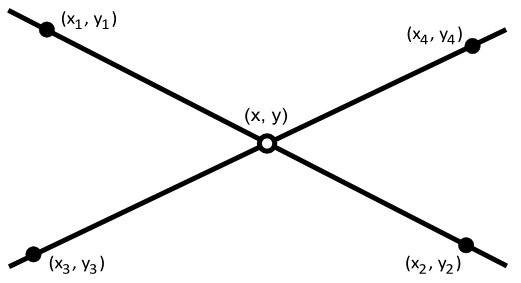
\includegraphics[height=2in]{Line-Line_Intersection.png}
%        \caption{Line line intersection}
%        \label{fig:linelineintersect}
%    \end{figure}
%}


 

\frontmatter 
\maketitle
\tableofcontents 
\chapter{Preface}

This book is intended as a reference, to be used both during the competition as well
in preparation for it.

It is hosted on github at
\href{https://github.com/VTACMProgrammingTeam/ICPCHandbook}{https://github.com/VTACMProgrammingTeam/ICPCHandbook}.
If you wish to contribute, please send email to godmar@gmail.com

The following authors have contributed to this book in its current form:
\begin{itemize}
    \item Godmar Back \texttt{<godmar@gmail.com>}
\end{itemize}
 

\mainmatter 
\chapter{String Processing}

\section{Regular Expressions}

\subsection{Regular Expressions}

\subsection{Zero-width Lookahead Technique}
\label{sec:lookaroundsplitting}

\begin{figure}
    \centering
    % Wikipedia Public Domain image
    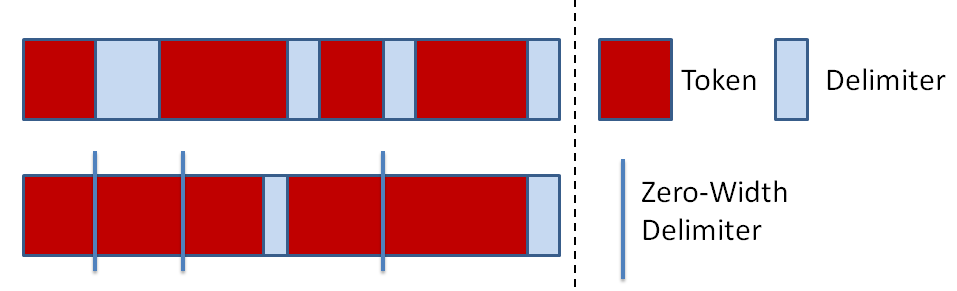
\includegraphics[height=1.5in]{lookaheadsplitting.png}
    \caption{Lookahead Splitting. The top shows a traditional scanner/split which consumes delimiters.
    The bottom shows a scanner using delimiter expressions that may or may not consume characters.}
    \label{fig:lookaheadsplit}
\end{figure}

In some problems (notably, 
      2007/B/Mobile~\ref{sec:2007-b-mobile}, 
      2007/D/Witness~\ref{sec:2007-d-witness}, 
      and 2008/G/Stems~\ref{sec:2008-g-stems}),
the string and/or input handling of these problems can greatly 
benefit from using zero-width positive lookahead/lookbehind regular expressions.

To understand how they work, consider how java.util.Scanner works. By
default, a Scanner splits the input stream into tokens using a delimiter
pattern. The default delimiter pattern is one or more whitespaces
(written as \verb!\p{javaWhitespace}! or, when embedded in Java code, as
\verb!"\\p{javaWhitespace}+"!). The input characters that are matched by the
delimiter itself are consumed by the Scanner – there is no way to
retrieve them.

In some cases, whitespace is not a suitable delimiter. Suppose
you're asked to parse an arithmetic expression that uses +, -, *,
and /. Whitespaces are optional, so both \verb!1+1! and \verb!1 + 1! as well as 
\verb!1 +1! are valid expressions. If you made the operators '+', '-'
etc. delimiters (perhaps in addition to whitespace), a Scanner would
retrieve '1' and '1', but there would be no way to retrieve the
'+' – so you couldn’t distinguish '1+1' and '1-1'.  Instead, use
lookaround matching by adding a zero-width delimiter that matches before
or after a +, -, *, or /.  ``Zero-width'' here means that although
the delimiter matches (and thus causes the Scanner to stop and return
what it has read so far!), it does not consume any characters. Thus,
the scanner will stop, but the delimiter (which the Scanner swallows)
has zero width – therefore, the characters are returned as part of
the previous token. In this example, s.next() would return '+'.

Figure~\ref{fig:lookaheadsplit} shows a traditional scanner (top) and a scanner that
uses both consuming and non-consuming delimiters (bottom): Note that
if the delimiter used by the scanner does not consume any characters,
the scanner will return the entire input stream. This is very useful if
you need to manipulate a stream without losing any characters.

The idea to use String.format to turn any regular expression into a 
zero-width lookahead or lookbehind delimiter is taken from \href{http://stackoverflow.com/questions/2206378/how-to-split-a-string-but-also-keep-the-delimiters}{here}.

Note that this technique can be used with a java.util.Scanner object
(via useDelimiter), but also in all other functions that use regular
expressions as delimiters, notably String.split().

Finally, note that you cannot use some regular expressions to describe
zero-width delimiters. Notably, \textbf{expressions using repetition (* or +)
cannot be used.}

\paragraph{Code Example.}
The following program shows some of the applications of
this style of matching.  These examples include:
\begin{itemize}
\item Arithmetic expressions with optional whitespace
\item S-Expressions with optional whitespace before and after ( )
\item Finding words in a sentence
\item Finding sentences in a paragraph
\end{itemize}

\inputminted{java}{code/Lookaround.java}

\subsection{NFA Simulation}
\index{NFA!Simulation}

The Regex engine in Java does not convert to a Thompson-DFA; it uses a backtracking algorithm
to find out if a regular expression matches a string.  This leads to pathological cases with
exponential runtime increase, particularly when the regular expression contains a large number
of Kleene stars.

In those situations, it may be helpful to construct your own mini-regexp interpreter by building
and simulating an NFA (nondeterministic finite automaton).

Example problem is \href{http://ncpc.idi.ntnu.no/ncpc2011/ncpc2011problems.pdf}{NCPC 2011/E}
where the input are globs such as \texttt{*a*a*a*a} that should be matched against filenames.
Figure~\ref{fig:nfaexample} shows an example of how to construct such a NFA.
In an NFA there may be multiple transitions labeled with the same symbol: for instance,
there's a transition labeled 'b' from state 0 to state 1, but there is also a transition
labeled 'b' from state 0 to state 0.  For the input string \texttt{abc}, the 'b' would
transition into state 1, whereas for the input string \texttt{abbc}, the first 'b' would
transition into state 0, the second into state 1.

Of course, we don't know which it's actually going to be - a NFA, in its theoretical 
formulation, is defined to oracle-like pick the correct transition.  That's why we simulate
it by simply keeping track of all possible (``active'') states the NFA might be in after each symbol.
This is done using a set (HashSet or BitSet if the states are nicely numbered).
For each input symbol, we compute the possible set of successor states based on the
current set of active states.  If after the string has been exhausted the goal state
is in the set of active states the string is matched.
A Python solution is shown below for succinctness.

\begin{figure}
    \centering
    % Wikipedia Public Domain image
    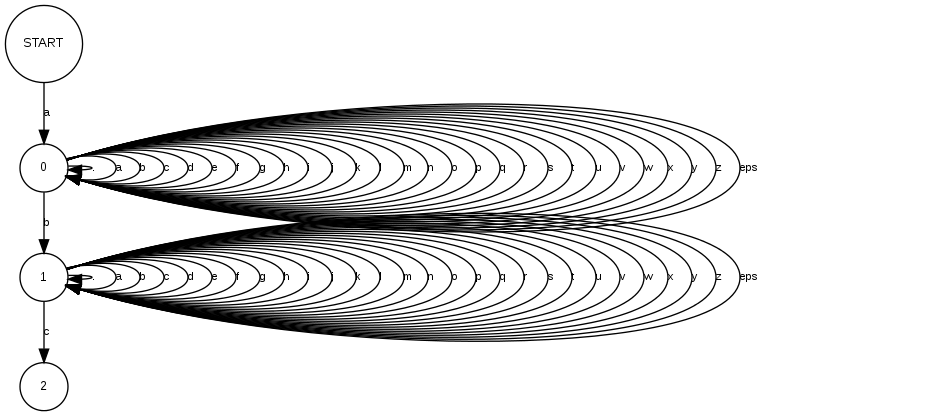
\includegraphics[height=3in]{a-star-b-star-c.png}
    \caption{NFA for regular expression \texttt{a.*b.*c} representing glob \texttt{a*b*c}
        over alphabet of lowercase letters and period (.)}
    \label{fig:nfaexample}
\end{figure}

\inputminted{python}{code/ls.py}

\section{Parsing}
\subsection{Recursive Descent}

 
\chapter{Geometry}

\section{Basics}

A determinant of a $2x2$ matrix is defined as
\[
    \left\vert
        \begin{array}{cc}
            a & b \\
            c & d \\
        \end{array}
    \right\vert
    = a d - b c
\]

\section{java.awt.geom}

The \texttt{java.awt.geom} and \texttt{java.awt} packages have, albeit limited, facilities
for geometric problems.  There are classes to represent shapes - see
\href{http://docs.oracle.com/javase/6/docs/api/java/awt/Shape.html}{java.awt.Shape}, including
lines, ellipses, rectangles and some curves.

\begin{itemize}
\item "is contained in".  java.awt.geom.Shape provide a contains() method to test if a point
    is contained in a shape.  Contains() returns true if the point is in the interior, and false
    if the point is outside the shape. However, it \textbf{may return true or false if the point is 
    on the shape boundary.} 

\begin{figure}
    \centering
    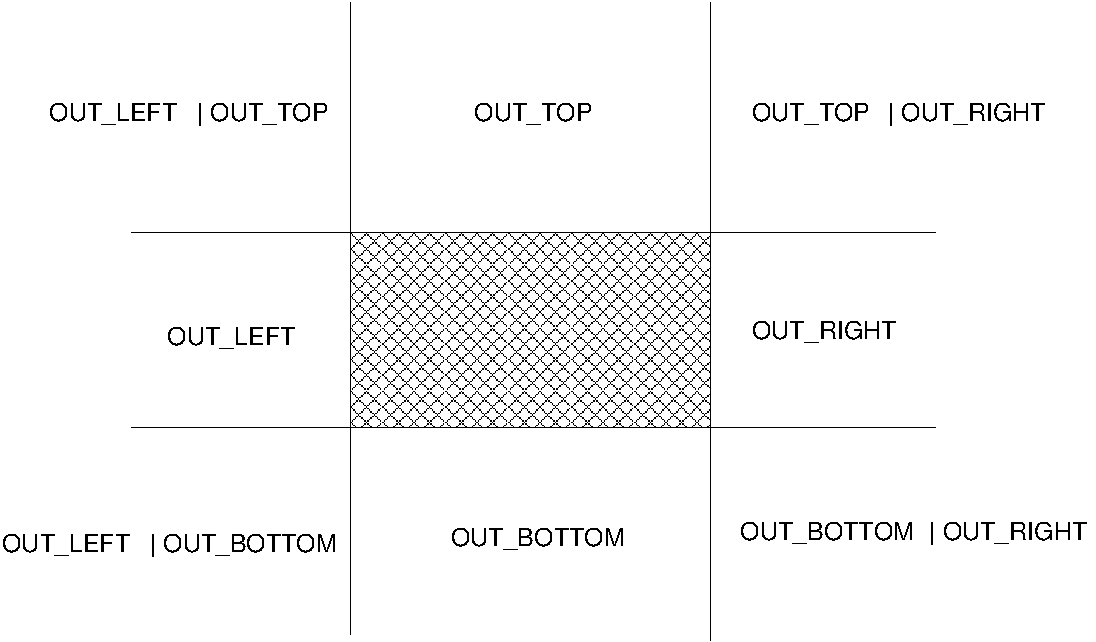
\includegraphics[height=2in]{outcode.pdf}
    \caption{Outcode - note that points that lie on any of the sidelines are considered inside.}
    \label{fig:outcode}
\end{figure}

\item "outcode". Outcodes were invented by Cohen-Sutherland; they are used for clipping
    in computer graphics.  java.awt.geom.Rectangle2D provides an outcode() method.
    The result is 0 if a point is inside or on any sideline of the rectangle; otherwise 
    the result is a
    combination of bits that represent where the point lies in relationship to the
    rectangle, as shown in Figure~\ref{fig:outcode}.
    For clipping of lines, the outcodes of the start and end point are
    computed, which then allows a quick identification of whether the line is inside,
    must be clipped, may be ignored, or needs further investigation.
    A useful property of outcode() is that it can substitute as a replacement for
    contains() in case where a point may lie on an edge but should be considered
    inside. 

\item "intersects."  Tests if a shape intersects with a rectangle.
    Can also test if two lines or line segments intersect, but cannot find the point of
    intersection.

\item "is point on line segment." Implements this as Line2D.ptSegDistSq(Point2D) $<$ 1e-9.

\end{itemize}

\section{Coordinate Geometry}

\subsection{Line/Line Intersection}
\label{sec:lineintersection}
\index{Line/Line Intersections}

\begin{figure}
    \centering
    % Wikipedia Public Domain image
    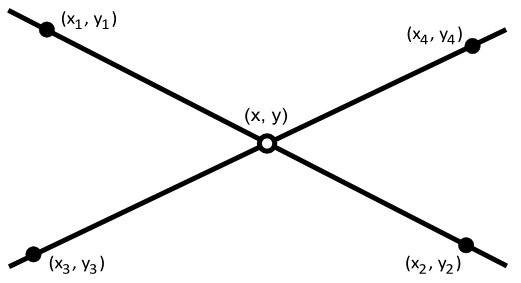
\includegraphics[height=1.5in]{Line-Line_Intersection.png}
    \caption{Line line intersection}
    \label{fig:linelineintersect}
\end{figure}

\[
\begin{array}{ll}
P_x = \frac{\begin{vmatrix} 
                \begin{vmatrix} x_1 & y_1\\
                                x_2 & y_2
                \end{vmatrix} & 
                \begin{vmatrix} x_1 & 1\\
                                x_2 & 1
                \end{vmatrix} \\\\ 
                \begin{vmatrix} x_3 & y_3\\
                                x_4 & y_4
                \end{vmatrix} & 
                \begin{vmatrix} x_3 & 1\\
                                x_4 & 1
                \end{vmatrix} 
            \end{vmatrix} }{
            \begin{vmatrix} 
                \begin{vmatrix} x_1 & 1\\
                               x_2 & 1
                \end{vmatrix} &  
                \begin{vmatrix} y_1 & 1\\
                                y_2 & 1
             \end{vmatrix} \\\\ 
             \begin{vmatrix} x_3 & 1\\
                             x_4 & 1
             \end{vmatrix} & 
             \begin{vmatrix} y_3 & 1\\
                             y_4 & 1 
             \end{vmatrix} 
            \end{vmatrix}}

&

P_y = \frac{\begin{vmatrix} 
                \begin{vmatrix} x_1 & y_1\\
                                x_2 & y_2
                \end{vmatrix} &  
                \begin{vmatrix} y_1 & 1
                              \\y_2 & 1
                \end{vmatrix} \\\\ 
                \begin{vmatrix} x_3 & y_3\\
                                x_4 & y_4
                \end{vmatrix} & 
                \begin{vmatrix} y_3 & 1\\
                                y_4 & 1
                \end{vmatrix} 
            \end{vmatrix} }
           {\begin{vmatrix} 
               \begin{vmatrix} x_1 & 1\\
                               x_2 & 1
               \end{vmatrix} &
               \begin{vmatrix} y_1 & 1\\
                               y_2 & 1
            \end{vmatrix} \\\\ 
            \begin{vmatrix} x_3 & 1\\
                            x_4 & 1
            \end{vmatrix} & 
            \begin{vmatrix} y_3 & 1\\
                            y_4 & 1
            \end{vmatrix} 
     \end{vmatrix}}\,\!
\\

\end{array}
\]

The determinants can be written out as:
\begin{align*}
    (P_x, P_y)= \bigg(&\frac{(x_1 y_2-y_1 x_2)(x_3-x_4)-(x_1-x_2)(x_3 y_4-y_3 x_4)}{(x_1-x_2)(y_3-y_4)-(y_1-y_2)(x_3-x_4)}, \\
                      &\frac{(x_1 y_2-y_1 x_2)(y_3-y_4)-(y_1-y_2)(x_3 y_4-y_3 x_4)}{(x_1-x_2)(y_3-y_4)-(y_1-y_2)(x_3-x_4)}\bigg)
\end{align*}

Source: \href{http://en.wikipedia.org/wiki/Line-line_intersection}{http://en.wikipedia.org/wiki/Line-line\_intersection}.

\paragraph{Notes}
\begin{itemize}
\item Does not handle parallel or coincident lines:
    Denominator will be zero:
    \[
        (x_1 - x_2) (y_3 - y_4) - (y_1 - y_2) (x_3 - x_4) = 0
    \]
\item Does not handle if lines are each others' normal (i.e., at a right angle).
    If line is horizontal ($y_1 = y_2$ or $y_3 = y_4$), and the other vertical ($x_1 = x_2$ or $x_3 = x_4$) 
    denominator will also be a 0 determinant, but the lines will intersect.  
    Handle as special case if problem allows it.

\item Intersection point may be outside the given segments.

\item If you only need to know if two lines intersect, but not where, use java.awt.geom.Line2D.intersects.
\end{itemize}

\paragraph{Code}

This code is from a solution to 2011/F (Section~\ref{sec:2011-f-lineofsight}) where the 
parallel and rectangular cases do not occur. (TBD: provide complete implementation.)

\inputminted[fontsize=\footnotesize,linenos=true]{java}{code/lineintersection.java}

%
%
%

\subsection{Area of a Polygon}
\label{sec:areapolygon}
\index{Polygon!Area}
\index{Area!Polygon}
\index{Polygon}

The signed area of a planar non-self-intersecting polygon with vertices $(x_1, y_1), \dots, (x_n, y_n)$ is
\[
    A = \frac{1}{2} \left(
        \left\vert
        \begin{array}{cc}
            x_1 & x_2 \\
            y_1 & y_2 \\
        \end{array}
        \right\vert
        +
        \left\vert
        \begin{array}{cc}
            x_2 & x_3 \\
            y_2 & y_3 \\
        \end{array}
        \right\vert
        + \ldots +
        \left\vert
        \begin{array}{cc}
            x_n & x_1 \\
            y_n & y_1 \\
        \end{array}
        \right\vert
        \right)
\]

Figure~\ref{fig:polygonareadeterminant} shows how to multiply this out
\[
    A = \frac{1}{2} \left(
        x_1 y_2 - x_2 y_1
      + x_2 y_3 - x_3 y_2
      + \ldots +
      + x_{n-1} y_n - x_n y_{n-1}
      + x_{n} y_1 - x_1 y_n
      \right)
\]

(Source: Mathworld~\cite{mathworldpolygonarea})

\begin{figure}
    \centering
    % Wikipedia Public Domain image
    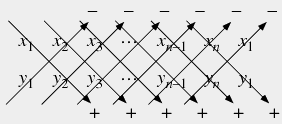
\includegraphics[height=1.5in]{PolygonArea_1000.png}
    \caption{Line line intersection}
    \label{fig:polygonareadeterminant}
\end{figure}

\paragraph{Notes}
\begin{itemize}
\item Works for any simple polygon (concave or convex)
\item Does not work for complex polygons (when any edges intersect)
\item Points \textbf{must be ordered} if polygon has more than 3 vertices, or output is junk.
\item A is positive if points are in counterclockwise order, negative if points are in clockwise order.
    See the use of Math.abs() in code below.
\item Triangle and any Quadrilateral are, of course, just special cases.
    For triangles, order does not matter.
\end{itemize}

\paragraph{Code}
\inputminted[fontsize=\footnotesize,linenos=true]{java}{code/polygonarea.java}

Special case of a triangle:

\inputminted[fontsize=\footnotesize,linenos=true]{java}{code/triangleareacoord.java}

 

\backmatter 
%\include{glossary} 
%\include{notat} 

\bibliographystyle{plain} %The style you want to use for references. 
\bibliography{references} %The files containing all the articles and books you ever referenced. 

\printindex

\end{document}

